\section{Distance estimates for main sequence stars in Ks filter}

\begin{figure*}

    \centering
    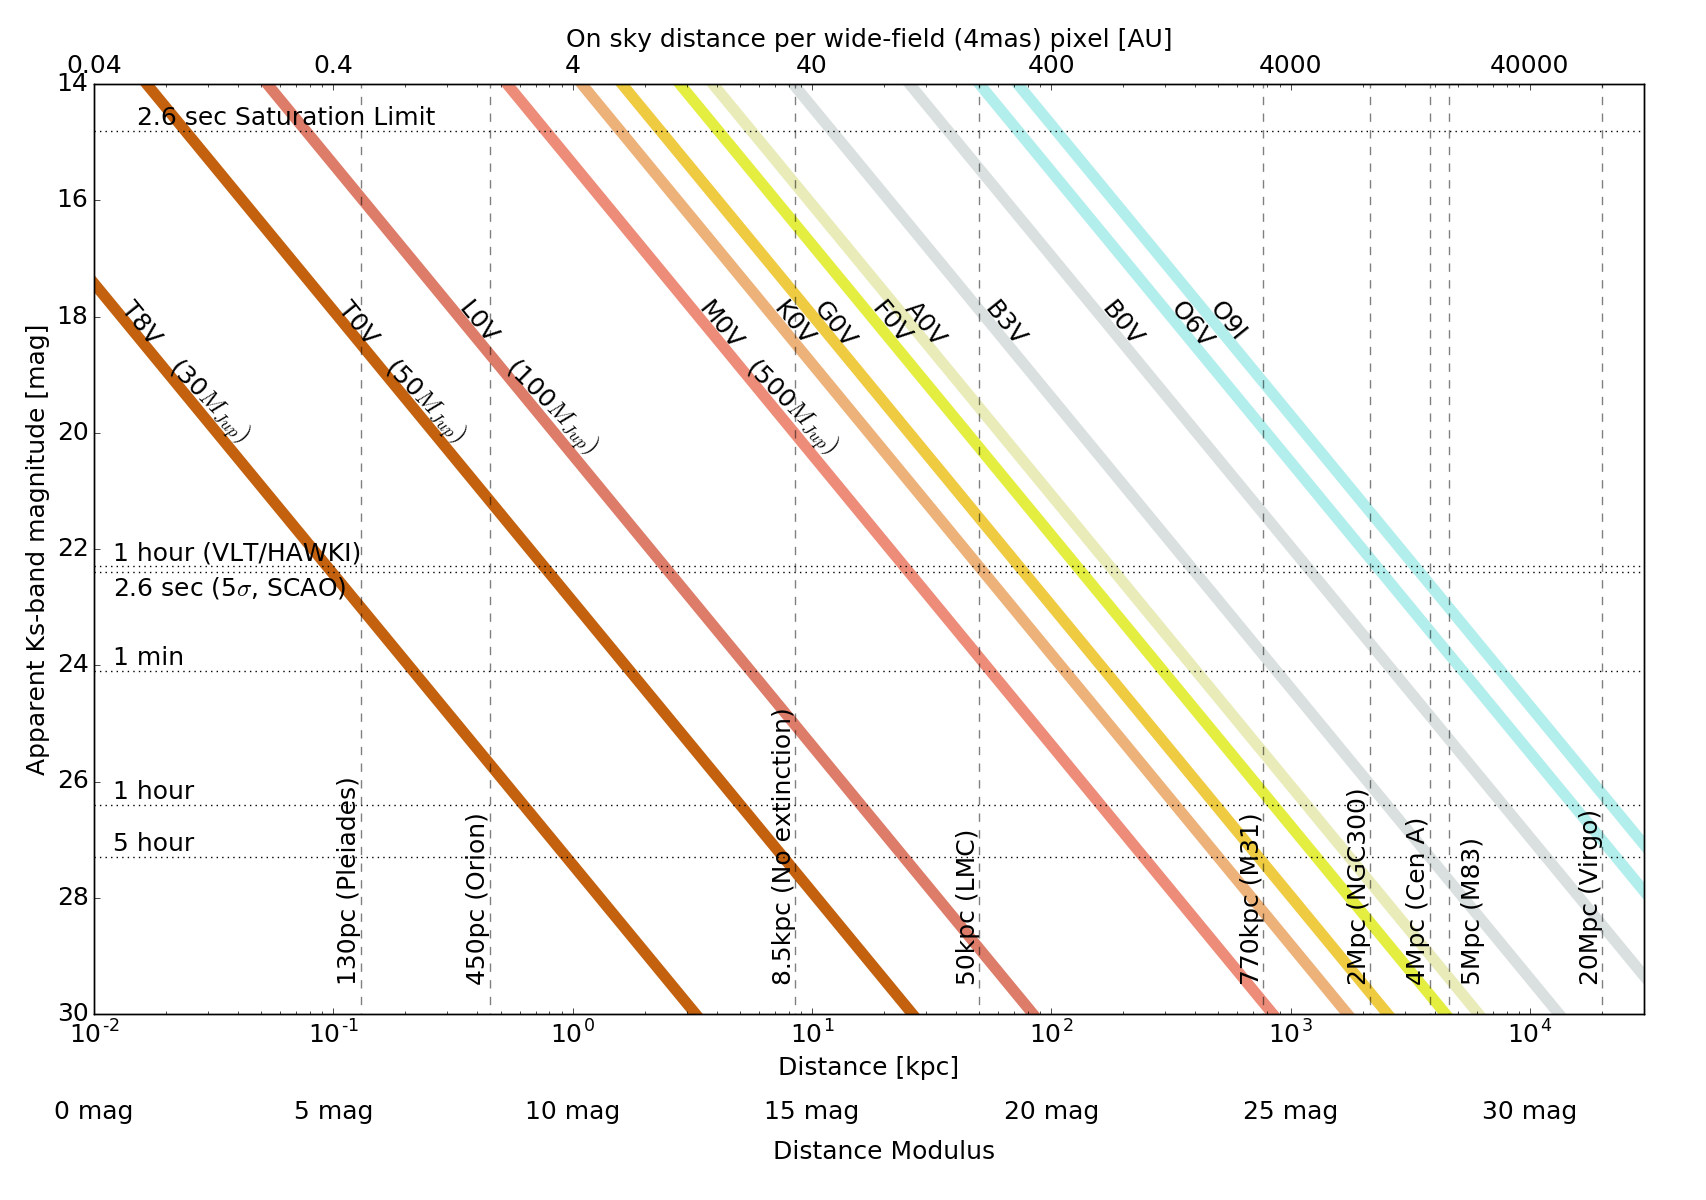
\includegraphics[width=\textwidth]{images/spec_type_vs_dist_paper2_Ks}
    
    \caption{The Ks-band equivalent of Fig.~\ref{fig:MS_distances}. As described in Fig.~\ref{fig:MS_distances} the coloured lines represent the apparent magnitude of the major spectral types with increasing distance. The dashed horizontal lines, unless otherwise stated, represent the $5\sigma$ detection limits for various exposure times with MICADO. When a coloured line crosses below a horizontal line, it means that this type of main sequence star will no longer be detectable by MICADO at the distance when the cross occurs. As a reference the dashed vertical lines show distances to well known astronomical objects.}
    
    \label{fig:MS_distances_Ks}
    
\end{figure*}


% \section{Comparison of the HAWK-I and MICADO configuration files}

% Although the SimCADO package is in the public domain, it currently does not have a software licence. Nevertheless we encourage anyone interested in simulating future ELT/MICADO observations to use SimCADO and to report any bugs to the authors. In the interests of transparency and reproducibility, we have included the configuration files that we used to generate SimCADO models of both the HAWK-I and MICADO optical trains. We are also willing to share any of the data files that subsequent users may need in order to reproduce our results. Please contact the authors directly. The software can be found at \url{www.univie.ac.at/simcado}


% \subsection{The MICADO configuration file}
% \label{appendix:micado_config}

% The standard configuration file used for the MICADO wide-field (4\,mas plate scale) imaging mode.

% \input{images/default.config}


% \subsection{The HAWKI configuration file}

% Rather than listing the full configuration for SimCADO as in Sect.~\ref{appendix:micado_config}, we simply list the parameters that were changed in order to create an optical train for UT4/HAWKI at the VLT.

% \input{images/hawki.config}


% \section{Settings for the HxRG Noise Generator script}

% In order to generate a stack of noise frames, SimCADO uses the python package NGHxRG. We have modified the values to reflect the characteristics of the new HAWAII-4RG chips that will be used in MICADO. The settings used by SimCADO are listed below:


% \begin{table*}
    % \centering
    % \begin{tabular}{|l|c|l|}
        % \hline
        % Noise Parameter             & Default Value & Description \\
        % \hline
        % White noise                 & 4 e-  & Standard deviation of read noise in electrons \\
        % Correlated pink noise       & 3 e-  & Standard deviation of correlated 1/f noise \\
        % Uncorrelated pink noise     & 1 e-  & Standard deviation of correlated 1/f noise \\
        % Alternating column noise    & 0.5 e$^-$ & Standard deviation of alternating column noise \\
        % Pedestal noise              & 4   e$^-$ & Level of pedestal drift in electrons \\
        % Number of read out channels & 64    &  \\
        % Number of row overheads     & 8     &  \\
        % Dead pixels                 & 1\%   & Percentage of pixels that are either ''hot'' or dead \\
        % Dead lines                  & 1\%   & Percentage of lines that are either ''hot'' or dead \\
        % \hline
    % \end{tabular}
    
    % \caption{Settings used by the HxRG noise generator code to model the read-out noise of the future MICADO detectors. See \citet{nghxrg} for more details.}
    % \label{tab:nghxrg}
    
% \end{table*}

